\section{Literature Review and Hypotheses}\label{sec:lit}

\subsection{Digital Factor Allocation and Regional Coordinated Development}

Regional coordinated development refers to the joint improvement of economic performance, social welfare, and urban-rural balance across regions, not simply the convergence of GDP per capita. It also requires that public services, income opportunities, and basic infrastructure be accessible in different locations and that the gains from growth be shared between leading and lagging areas \citep{kanbur2005,worldbank2009}. In China, RCD has been pursued through fiscal transfers, infrastructure investment, poverty alleviation, and, more recently, digitalization.

DFA can affect RCD through four channels. Digital infrastructure reduces communication and transaction costs, allowing firms in lagging regions to reach customers and information that were previously available only in core regions \citep{czernich2011,hjort2019}. Digital finance extends payment, savings, credit, and insurance to households and small firms, improving risk sharing and relaxing liquidity constraints \citep{jack2014,beck2007,liu2023}. Digital industry creates new tasks and raises productivity in services that are less dependent on physical distance \citep{goldfarb2019,acemoglu2011}. Digital human capital determines whether local workers can use digital tools productively \citep{akerman2015,vandijk2005}.

This reasoning supports a positive relationship, but the empirical literature also cautions that the benefits are conditional. Forman et al. (2012) show that the internet's wage effects are concentrated in already prosperous areas, and Akerman et al. (2015) find that broadband complements skilled labor. Whether DFA has a uniform effect across Chinese regions is therefore an open question.

\subsection{Absorptive Capacity and Threshold Effects}

The idea that digitalization has stage-dependent effects comes from the absorptive-capacity literature. Digital technologies are general-purpose technologies whose effects depend on how they are combined with organizational change, human capital, and institutional quality \citep{brynjolfsson2014,omahony2005}. In low-income regions with thin markets, digital inputs may be used for consumption rather than productive investment; in higher-income regions the same inputs can be combined with skills, finance, and infrastructure to generate larger coordination gains. This predicts that the marginal effect of DFA increases with economic development.

Hansen (1999) provides a fixed-effects panel threshold estimator that lets the slope of a regressor differ across regimes defined by an observed variable, searching for the threshold that minimizes the residual sum of squares and testing linearity by bootstrap. The approach has been extended to instrumental-variable and dynamic panels \citep{caner2004,seo2016} and is widely used on Chinese regional data. Qi et al. (2025), for example, find threshold effects of digital development, market efficiency, and technological progress on Chinese-style modernization, which suggests that the digital dividend depends on the broader development environment.

The threshold interpretation also connects to the digital divide. Access is only the first level; the second and third levels concern skills and the ability to convert access into material benefits \citep{vandijk2005,norris2001,warschauer2003}. If the second and third divides persist in low-income regions, the effect of DFA on RCD may be weak there and stronger once complementary capabilities are in place.

\subsection{Financial Development and Diminishing Returns}

Digital finance is a core component of DFA, and its effect may depend on the depth of the financial system. Where financial development is limited, digital finance substitutes for missing branches and expands access to basic services. Where the system is already deep, it adds less at the extensive margin, may intensify competition, or may divert resources from productive investment. The relationship between financial depth and inclusion is therefore unlikely to be linear \citep{beck2007}. Digital finance has expanded fastest in leading cities where financial services were already abundant, so its marginal contribution to RCD may be larger where finance is scarce. This motivates a second threshold in financial development.

\subsection{Regional Heterogeneity and Mechanisms}

China's regions differ in initial digital endowments, industrial structure, and institutional capacity. The east has denser digital infrastructure, more high-skilled labor, and deeper financial markets; the centre and west start lower but may have more room for catch-up; the northeast carries a heavy-industry legacy and a slow digital transition. The absorptive-capacity argument predicts a stronger effect in the east, whereas the catch-up argument predicts a stronger effect in the west. The two can be distinguished empirically.

Three mechanisms are relevant. DFA can promote industrial upgrading by reducing information costs, expanding market access, and enabling new service activities \citep{chen2025,rodrik2016}. It can deepen financial development by extending the coverage and use of digital financial services \citep{chen2025,liu2023}. And it can raise technological investment by lowering the cost of innovation-related information and creating demand for digital skills \citep{akerman2015}. The channel analysis in this study is exploratory.

\subsection{Hypotheses}

\textbf{H1.} Digital factor allocation is positively associated with regional coordinated development.

\textbf{H2.} The effect of DFA on RCD is nonlinear; the marginal effect is larger after economic development crosses a threshold, consistent with absorptive capacity.

\textbf{H3.} The effect of DFA varies with financial development and tends to diminish at very high levels of financial depth.

\textbf{H4.} The effect of DFA is regionally heterogeneous, with a stronger average effect in less-developed western provinces.

\textbf{H5.} DFA promotes RCD through industrial upgrading, financial deepening, and technological investment.

\begin{figure}[H]
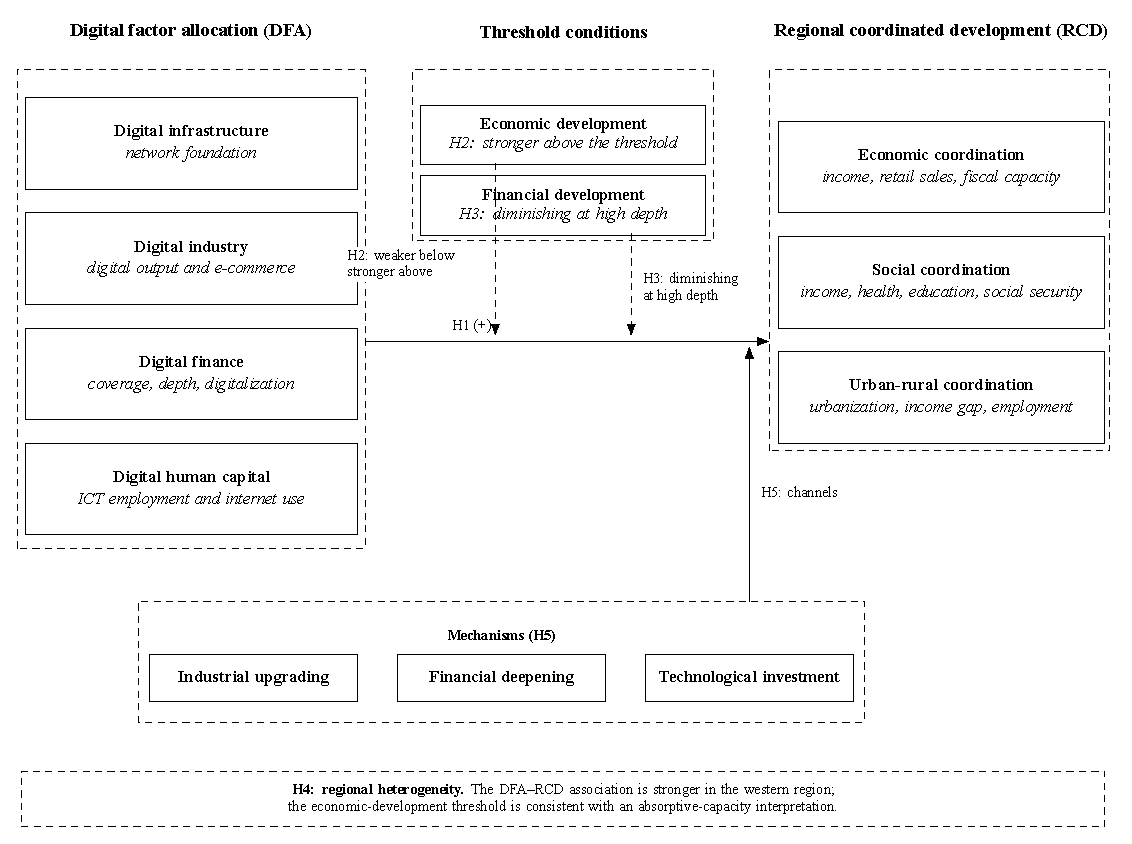
\includegraphics[width=0.95\textwidth]{figures/fig1_framework_tikz.pdf}
\caption{Research framework. DFA is measured across four dimensions and RCD across three dimensions. H1 tests the average association; H2 tests whether the DFA slope differs across economic-development regimes; H3 examines the financial-development threshold; H4 summarizes regional heterogeneity; H5 examines the channels.}\label{fig:framework}
\end{figure}
